\chapter{Experiment 1 - Dataset and in-Network Transformation of MNIST}
\label{chap:five}

\section{Motivation}
In order to contextualize the results of the experiments we wish to conduct on malware data, we consider the methods presented there on the well-studied MNIST Database of Handwritten Digits~\cite{lecun1998mnist}.
MNIST is a benchmark in computer vision - since our baseline convolutional neural network is based on LeNet~\cite{lecun1998gradient}, we have a large body of research to compare to.
Additionally, MNIST serves as an introduction to the field of computer vision for many students and so our architectures and theories can be made more accessible in that context.
The current state of the art for MNIST~\cite{byerly2020branching}, achieved in January of this year achieves a 99.84\% accuracy.
The best results achieved in the original LeCun paper was 99.3\% accuracy and generally an accuracy greater than 98\% is considered to be good.

\section{Methodology}
In order to maintain consistency with our other findings, our methodology is identical to experiments in \ref{chap:three} and \ref{chap:four}, leveraging the same hardware as in \ref{append:one} and the same model details as in \ref{append:two}.
In this case, our dataset differs from our previous two experiments by virtue of being a ``true'' image dataset. 
As a result, some preprocessing work was required to reshape our 32 x 32 images into a flat vector, this is done without loss of information.

\section{models}
All code\footnote{Code is available at the following url: \url{https://github.com/erickgalinkin/jhu_masters}} was written in Python, using the Tensorflow 2, PyTorch, and Scikit-learn libraries.
Only the baseline models described in \ref{other models} used the Scikit-learn library, and only the Wavelet Convolutional network described in \ref{wavelet cnn} used PyTorch.
The remaining models all used the Tensorflow framework.

\subsection{Fully-Connected Neural Network}
The fully-connected neural network architecture accepts, as input, a 1x100 row-vector.
This vector is then fed to three densely connected layers, each with 256 ReLU-activated neurons.
The output neuron is a single sigmoid-activated neuron, which provides a probability of traffic being benign.

\subsection{Standard Convolutional Neural Network}
Our standard convolutional neural network is a sequential model which accepts the same sort of input as our fully-connected neural network, and passes it to an architecture comprised of two convolution and max-pooling blocks, followed by batch normalization, and then passed to two densely connected layers of 128 neurons each. The architecture is visualized below in figure \ref{fig:conv net}.

\begin{figure}[ht]
\caption{Convolutional Neural Network Architecture}
\label{fig:conv net}
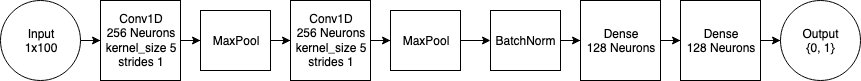
\includegraphics[width=\textwidth]{conv_architecture}
\centering
\end{figure}

\subsection{Other Models} \label{other models}
Two baseline models were considered.
The first is the random forest model provided in the Scikit-learn library with no hyperparameter tuning.
Decision tree models are generally good at classification tasks~\cite{hastie01statisticallearning} but are weak classifiers which are sensitive to variance.
Random forests are a the result of averaging a large collection of de-correlated trees and provide a good benchmark as a na\"ive model - in the respect that it is untuned - for classification.

The other benchmark model is a Support Vector Classifier, again provided by the Scikit-learn library.
The rationale for using a Support Vector Machine is that we wanted to see if some hyperplane could be learned which would separate the data.
This model was again, na\"ive in the respect that it was merely the ``out of the box'' model, and so the classifier was built on top of the radial basis function kernel.

\section{Results}

\begin{table}[h]
\caption{Neural Network Results}
\centering
\label{Tab:test}	
\begin{tabular}{l|ll}
\textbf{Data and Architecture}  & \textbf{Test Accuracy} & \textbf{Mean Step Time} ($\mu$s) \\\cline{1-3}
Raw, Fully-Connected NN            & 97.73\%         & 29\\
Fourier, Fully-Connected NN        & 98.12\%         & 41\\
Wavelet, Fully-Connected NN        & 97.83\%         & 30\\
\hline
Raw, Convolutional NN              & 99.11\%         & 204\\ 
Fourier, Convolutional NN          & 99.10\%         & 237\\
Wavelet, Convolutional NN          & 99.10\%         & 212\\
\hline
Raw, Fourier NN                    & 98.45\%         & 959\\
Raw, Wavelet NN                    & 98.89\%         & 1068\\ 
\end{tabular}
\end{table}

In this case, all of our models achieve accuracy over 97\% which is broadly considered to be the benchmark accuracy for MNIST. 
For all these combinations of architecture and transformation, the difference between our maximum accuracy score of 99.11\% and our minimum accuracy of 97.73\% is only 1.38\%.
Comparing the convolutional models in particular, the difference between the Raw, Fourier-transformed, and Wavelet-transformed data is only 0.01\%. 